\section{Equações Diferenciais Ordinárias Rígidas}

\textbf{Definição:} Equações Diferenciais Ordinárias são ditas rígidas quando a solução é uma função suave, mas requer um \esp{ \Delta t } muito pequeno no método numérico para manter estabilidade.

Por exemplo,

\begin{equation}
 \label{cap6:sec5:eq1}
 \left\{
 \begin{array}{ll}
  y'       & = - \alpha \, y + s \, (t) \\
  y \, (0) & = y_0
 \end{array}
 \right.
\end{equation}

\esp{ \displaystyle \frac{1}{|\alpha|} } denominada ``constante de tempo''.\\

Solução exata de \ref{cap6:sec5:eq1} :

\begin{itemize}

\item Se
\begin{eqnarray}
 && s \, (t) = 0 \qquad \forall \, t \nonumber \\
 \label{cap6:sec5:eq2}
 && y \, (t) = y_0 \, e^{-\alpha \, t}
\end{eqnarray}

\item Se
\begin{eqnarray}
 && s \, (t) \neq 0 \nonumber \\
 \label{cap6:sec5:eq3}
 && y \, (t) = y_0 \, e^{-\alpha \, t} + e^{-\alpha \, t} \, \int^t_0 s \, (\xi) \, e^{\alpha \, \xi} \, d\xi
\end{eqnarray}

\end{itemize}

OBS: A solução de problemas de E.D.O. rígidas pelos métodos de Runge-Kutta ou Preditor-Corretor são difíceis ou, às vezes, impossível.\\

Se aplicarmos o método de Runge-Kutta de quarta-ordem ao problema \ref{cap6:sec5:eq1} a solução se torna instável para \esp{ h > 2.785 \, \displaystyle \frac{1}{|\alpha|} }. Assim, quando \esp{ \displaystyle \frac{1}{|\alpha|} \rightarrow 0 } o método tem de utilizar \esp{ h \rightarrow 0 } para manter a estabilidade. Por exemplo, para

\[
 \alpha = -100000 \Rightarrow h < \frac{2.785}{100000} = 0.000002785 \, \times \, 10
\]

só para manter a estabilidade.

\begin{figure}[htb]
 \centering
 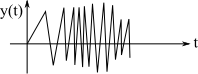
\includegraphics[scale=1.0]{capitulos/capitulo6/figuras/equa_dif_ord_rig1.png}
 \caption{?}
 \label{fig:equa_dif_ord_rig1}
\end{figure}

OBS: Se em um sistema de E.D.O.'s uma E.D.O. é rígida, \esp{ \Delta t } tem de ser pequeno para manter estabilidade da solução do sistema.

\begin{equation}
 \label{cap6:sec5:eq4}
 \left\{
 \begin{array}{l}
  y' = -1 \, y + 1 \, z + 3 \\
  z' = -10^7 \, z + 1 \, y \qquad \Rightarrow \displaystyle \frac{1}{|\alpha|} = \frac{1}{10^7} \qquad \mbox{(muito pequeno)}
 \end{array}
 \right.
\end{equation}

Alguns métodos para solução de E.D.O.'s rígidas utilizando \esp{ \Delta t } grande, foram propostos.

\subsection{Métodos Implícitos}

\begin{equation}
 \label{cap6:sec5:eq5}
 \left\{
 \begin{array}{l}
  y' = f \, (y, \, z, \, t) \\
  z' = g \, (y, \, z, \, t)
 \end{array}
 \right.
 \qquad
 \mbox{com}
 \left\{
 \begin{array}{l}
  y \, (0) = y_0 \\
  z \, (0) = z_0
 \end{array}
 \right.
\end{equation}

Usando \textit{Backward} Euler

\begin{equation}
 \label{cap6:sec5:eq6}
 \left\{
 \begin{array}{l}
  y_{n+1} - y_n = h \, f \, (y_{n+1}, \, z_{n+1}, \, t_{n+1}) \equiv h \, f_{n+1} \\
  z_{n+1} - z_n = h \, g \, (y_{n+1}, \, z_{n+1}, \, t_{n+1}) \equiv h \, g_{n+1}
 \end{array}
 \right.
\end{equation}

Se \esp{f} e \esp{g} forem funções não-lineares, \ref{cap6:sec5:eq6} não pode ser resolvida de forma fechada (exata) e métodos iterativos, tais como o das substituições sucessivas, podem ser usados mas não são eficientes. Uma opção mais eficiente é linearizar as equações \ref{cap6:sec5:eq6} por expansão de Taylor.

\begin{equation}
 \label{cap6:sec5:eq7}
 \left\{
 \begin{array}{l}
  f_{n+1} = f_n + \displaystyle \frac{\partial f}{\partial y} \, \Delta y + \frac{\partial f}{\partial z} \, \Delta z + \frac{\partial f}{\partial t} \, \Delta t \\
  \\
  g_{n+1} = g_n + \displaystyle \frac{\partial g}{\partial y} \, \Delta y + \frac{\partial g}{\partial z} \, \Delta z + \frac{\partial g}{\partial t} \, \underbrace{\Delta t}_{\displaystyle h}
 \end{array}
 \right.
\end{equation}

\ref{cap6:sec5:eq7} $ \rightarrow $ \ref{cap6:sec5:eq6} $ \Rightarrow $

\begin{equation}
 \label{cap6:sec5:eq8}
 \underbrace{
 \left[
  \left[
   \begin{array}{cc}
    1 & 0 \\
    0 & 1 \\
   \end{array}
  \right]
  - h \,
  \left[
   \begin{array}{cc}
    \displaystyle \frac{\partial f}{\partial y} & \displaystyle \frac{\partial f}{\partial z} \vspace*{0.2cm} \\
    \displaystyle \frac{\partial g}{\partial y} & \displaystyle \frac{\partial g}{\partial z}
   \end{array}
  \right]
 \right]
 \,
 \left[
  \begin{array}{c}
   \Delta y \\
   \Delta z
  \end{array}
 \right]
 =
 \left[
  \begin{array}{l}
   h \, f_n + h^2 \, \displaystyle \frac{\partial f}{\partial t} \vspace*{0.2cm} \\
   h \, g_n + h^2 \, \displaystyle \frac{\partial g}{\partial t}
  \end{array}
 \right]
 }_{(resolve \, \, por \, \, elimina\mbox{\textit{\scriptsize{çã}}}o \, \, de\, \, Gauss)}
\end{equation}

ou

\begin{equation}
 \label{cap6:sec5:eq9}
 \underbrace{(I - h \, J) \, \Delta \bar{y} = \mbox{Lado direito}}_{(resolve \, \, por \, \, elimina\mbox{\textit{\scriptsize{çã}}}o \, \, de\, \, Gauss)}
\end{equation}

onde

\begin{itemize}

\item \esp{I =} Identidade

\item \esp{J =} Matriz Jacobiana

\item \esp{ \Delta \bar{y} =
\left\{
\begin{array}{c}
 \Delta y \\
 \Delta z
\end{array}
\right\}
}

\end{itemize}

OBS: Incondicionalmente estável.

\subsection{Método Exponencial}

\underline{Idéias Básicas}\\

Suponha

\begin{equation}
 \label{cap6:sec5:eq10}
 y' = f \, (y, \, t)
\end{equation}

onde \esp{f \, (y, \, t)} não inclui \esp{t} explicitamente. Adicionando-se \esp{c \, y} aos dois lados de \ref{cap6:sec5:eq10}, temos:

\begin{equation}
 \label{cap6:sec5:eq11}
 y' + c \, y = f \, (y, \, t) + c \, y
\end{equation}

onde \esp{c} é constante.

Multiplicando-se \ref{cap6:sec5:eq11} por \esp{e^{c\,t}}, temos

\begin{eqnarray}
 \label{cap6:sec5:eq12}
 y' \, e^{c\,t} + c \, y \, e^{c\,t} & = & [f \, (y, \, t) + c \, y] \, e^{c\,t} \\
 \nonumber \\
 \label{cap6:sec5:eq13}
 \frac{d}{dt} \, (y \, e^{c\,t}) & = & [f \, (y, \, t) + c \, y] \, e^{c\,t}
\end{eqnarray}

\begin{figure}[htb]
 \centering
 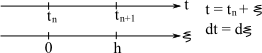
\includegraphics[scale=1.0]{capitulos/capitulo6/figuras/equa_dif_ord_rig2.png}
 \caption{Parametrização}
 \label{fig:equa_dif_ord_rig2}
\end{figure}

\begin{equation}
 \label{cap6:sec5:eq14}
 \int^{t_{n+1}}_{t_n} \left[ \frac{d}{d\eta} \, (y \, e^{c\,\eta}) \right] \, d\eta
 =
 \int^{t_{n+1}}_{t_n} \left[ f \, (y, \, \eta) + c \, y \right] \, e^{c\,\eta} \, d\eta
\end{equation}

\begin{equation}
 \label{cap6:sec5:eq15}
 y \, (t_{n+1}) \, e^{\,c\,t_{n+1}} - y \, (t_n) \, e^{\,c\,t_n} = \int^{\,h}_0 \, [f \, (y \, (t_n + \xi), \, t_n + \xi) + c \, y \, (t_n + \xi)] \, e^{\,c \, (t_n + \xi)} \, d\xi
\end{equation}

multiplicando-se por \esp{e^{-c\,t_{n+1}}}, temos

\begin{eqnarray}
 y \, (t_{n+1}) & = & y \, (t_n) \, e^{-c\,(t_{n+1}-t_n)} + \nonumber \\
 \label{cap6:sec5:eq16}
                & + & \int^{\,h}_0 \, [f \, (y \, (t_n + \xi), \, t_n + \xi) + c \, y \, (t_n + \xi)] \, e^{\,c \, (\xi - (t_{n+1} - t_n))} \, d\xi \\
 \label{cap6:sec5:eq17}
 y \, (t_{n+1}) & = & y \, (t_n) \, e^{-c\,h} + \int^{\,h}_0 \, [f \, (y \, (t_n + \xi), \, t_n + \xi) + c \, y \, (t_n + \xi)] \, e^{\,c \, (\xi - h)} \, d\xi
\end{eqnarray}

Vários métodos podem ser deduzidos utilizando-se aproximações para \esp{f + c \, y} no integrando de \ref{cap6:sec5:eq17}. No entanto, a precisão da aproximação vai depender do valor de \esp{\underline{c}}.

Uma aproximação de \esp{c} comumente utilizada é

\begin{equation}
 \label{cap6:sec5:eq18}
 c = \frac{\partial f}{\partial y} \, (t_n) = - \left( \frac{\partial f}{\partial y} \right)_n
\end{equation}

OBS: Quando \esp{f\,(y,\,t)} não tem dependência explícita de

\begin{equation}
 \label{cap6:sec5:eq19}
 \frac{\partial f}{\partial y} = \frac{f'}{f} \, \left( \frac{\partial f}{\partial t} ? \frac{\partial f}{\partial y} \, \frac{\partial y}{\partial t} = \frac{\partial f}{\partial y} \, f \right)
\end{equation}

Assim

\begin{equation}
 \label{cap6:sec5:eq20}
 c = - \left( \frac{f'}{f} \right)_n
\end{equation}

\subsection{Método de Ajuste Exponencial}

Aproximação:

\begin{equation}
 \label{cap6:sec5:eq21}
 [f \, (y, \, t_n + \xi) + c \, y \, (t_n + \xi)] \approx f_n + c \, y_n
\end{equation}

Equação \ref{cap6:sec5:eq17} reduz-se a

\begin{equation}
 \label{cap6:sec5:eq22}
 \underbrace{y_{n+1} = y_n + h \, f_n}_{Forward \, \, Euler} \, \left[\frac{1 - e^{-c\,h}}{c\,h}\right]
\end{equation}

OBS: O método \ref{cap6:sec5:eq22} é incondicionalmente estável

\[
 \begin{array}{lll}
  \mbox{Se } h \rightarrow 0 & \Rightarrow & y_{n+1} \rightarrow y_n , \, \mbox{ pois } 1 - e^{-c\,h} \rightarrow 0 \\
  \mbox{Se } h \rightarrow \infty & \Rightarrow & \left[ 1 - \displaystyle \frac{1}{e^{\,c\,h}} \right] \rightarrow 1
 \end{array}
\]

Modificação do método \ref{cap6:sec5:eq22} para melhorar a solução

\begin{enumerate}

\item Utilizar \ref{cap6:sec5:eq22} como um preditor

\begin{equation}
 \label{cap6:sec5:eq23}
 \bar{y}_{n+1} = y_n + f_n \, \left[ \frac{1 - e^{-c\,h}}{c} \right]
\end{equation}

ou no intervalo \esp{t_n < t < t_{n+1}}

\[
 \xi = t - t_n
\]

\begin{equation}
 \label{cap6:sec5:eq24}
 \bar{y} \, (t) = y_n + \left[ \frac{1 - e^{-c\,\xi}}{c} \right] \, f_n
\end{equation}

\item Reescrevemos \ref{cap6:sec5:eq17} como corretor

\begin{equation}
 \label{cap6:sec5:eq25}
 y_{n+1} = \bar{y}_{n+1} + \int^{\,h}_0 \, [f \, (\bar{y} \, (t_n + \xi), \, t_n + \xi) - f_n + c \, \bar{y} \, (t_n + \xi) - c \, y_n] \, e^{\,c(\xi?}
\end{equation}

A integral pode ser resolvida

\begin{enumerate}

\item Analiticamente (se \esp{f} for simples)

\item Interpolação linear de \esp{[ \, ]}

\item Regra do Trapézio

\end{enumerate}

interpolação linear

\begin{equation}
 \label{cap6:sec5:eq26}
 [f \, (\bar{y} \, (t_n + \xi)) - f_n + c\,\bar{y} \, (t_n + \xi) - c \, y_n] \approx B \, \xi
\end{equation}

onde

\begin{equation}
 \label{cap6:sec5:eq27}
 B = \frac{f_{n+1} - f_n + c \, (y_{n+1} - y_n)}{h}
\end{equation}

\begin{description}

\item[b)]
\begin{equation}
 \label{cap6:sec5:eq28}
 y_{n+1} = \bar{y}_{n+1} + \frac{B\,h^2}{c\,h} \, \left( \frac{1 - e^{-c\,h}}{c\,h - 1} \right)
\end{equation}

\item[c)]
\begin{equation}
 \label{cap6:sec5:eq29}
 y_{n+1} = \bar{y}_{n+1} + \frac{B\,h^2}{2}
\end{equation}

\end{description}

\end{enumerate}
